\chapter{Architecture 3 tiers}

\section{Architecture 3 tiers}

L'architecture Destiny Raid Companion suit une approche 3-tiers classique avec séparation nette entre présentation (Next.js), logique métier (Express.js) et données (PostgreSQL/Redis). Cette séparation permet une maintenance simplifiée, une scalabilité indépendante de chaque couche et une meilleure testabilité.

\begin{figure}[h]
    \centering
    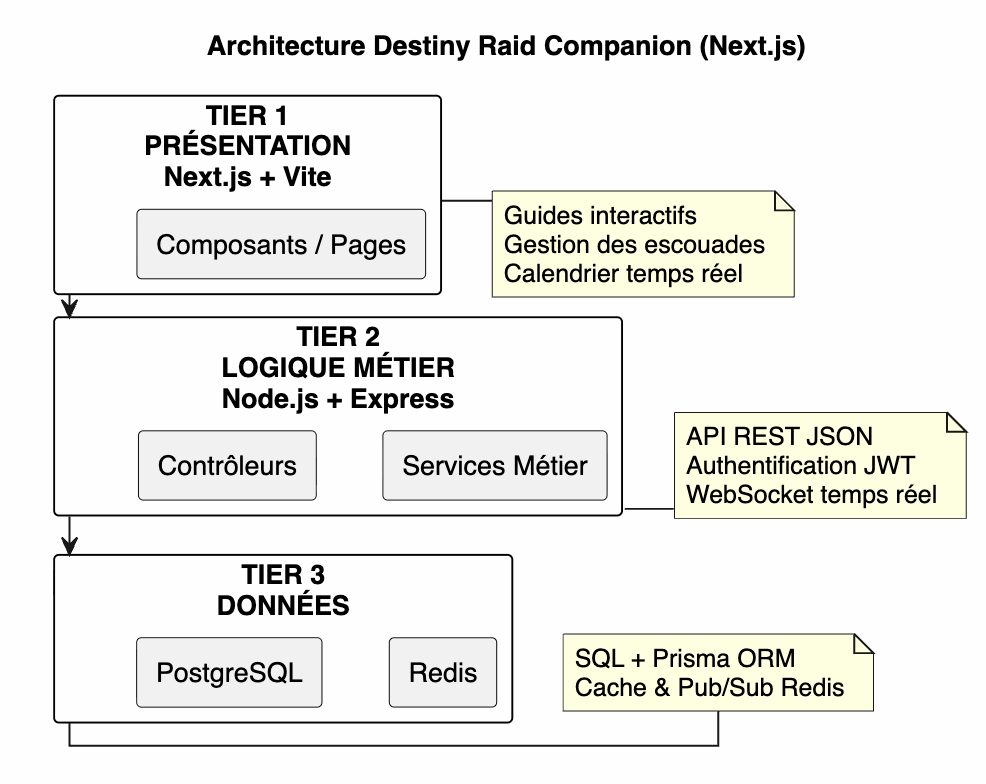
\includegraphics[width=0.6\textwidth]{assets/architecture_destiny.png}
    \caption{Architecture 3 tiers de Destiny Raid Companion}
    \label{fig:3tiers}
\end{figure}

\subsection{Couche Présentation (Next.js)}

Le frontend est développé avec Next.js 14 et TypeScript. J'ai choisi Next.js pour plusieurs raisons :

\begin{itemize}
    \item \textbf{Server-Side Rendering (SSR) :} Les guides de raids peuvent être pré-rendus côté serveur, ce qui les rend indexables par les moteurs de recherche et plus rapides à l'affichage initial.
    \item \textbf{App Router :} Structure de routage intuitive basée sur les fichiers.
    \item \textbf{Image Optimization :} Optimisation automatique des images, cruciale pour les illustrations des raids.
\end{itemize}

\subsubsection*{Structure simplifiée}

\begin{verbatim}
frontend/
+-- app/
|   +-- (dashboard)/           # Routes principales
|   |   +-- guides/[raidId]/   # Affichage d'un guide (SSR)
|   |   +-- squads/            # Gestion des escouades
|   +-- api/                   # API Routes (callbacks OAuth)
+-- components/                # Composants réutilisables
+-- middleware.ts              # Protection des routes
\end{verbatim}

\subsection{Couche Logique Métier (Express.js)}

Le backend utilise Node.js avec Express.js, structuré selon le pattern Controller-Service-Repository. \textbf{L'idée est de garder le code testable et de pouvoir faire évoluer la logique sans tout casser.}

\subsubsection*{Organisation des responsabilités}

\begin{itemize}
    \item \textbf{Controllers :} Gèrent les requêtes HTTP, valident les entrées, renvoient les réponses
    \item \textbf{Services :} Contiennent la logique métier (règles de l'application)
    \item \textbf{Repositories :} Accès à la base de données, isolation de Prisma
\end{itemize}

\paragraph{Exemple : création d'une escouade}

Le contrôleur reçoit la requête, valide les données avec Zod, puis appelle le service :

\begin{lstlisting}[language=JavaScript]
const createSquad = async (req, res, next) => {
  const validation = squadSchema.safeParse(req.body);
  if (!validation.success) {
    return res.status(400).json({ error: 'Données invalides' });
  }
  const squad = await squadService.createSquad(validation.data, req.user.id);
  res.status(201).json({ success: true, data: squad });
};
\end{lstlisting}

Le service applique les règles métier. Ici, deux règles importantes :
\begin{enumerate}
    \item Une escouade ne peut pas dépasser 12 membres
    \item Un joueur ne peut pas créer plus de 5 escouades
\end{enumerate}

La transaction Prisma garantit que l'escouade et l'ajout du leader comme membre sont créés ensemble, sans risque d'incohérence.

\begin{lstlisting}[language=JavaScript]
class SquadService {
  async createSquad(squadData, leaderId) {
    // Règles métier
    if (squadData.maxMembers > 12) {
      throw new BusinessError('Maximum 12 membres');
    }
    const userSquadCount = await this.squadRepository.countByUser(leaderId);
    if (userSquadCount >= 5) {
      throw new BusinessError('Limite de 5 escouades atteinte');
    }

    // Transaction pour garantir l'intégrité
    return await this.db.transaction(async (trx) => {
      const squad = await this.squadRepository.create(trx, {
        ...squadData,
        leader_id: leaderId
      });
      await this.squadMemberRepository.create(trx, {
        squad_id: squad.id,
        user_id: leaderId,
        role: 'leader'
      });
      return squad;
    });
  }
}
\end{lstlisting}

L'intérêt de cette séparation est concret : si demain la règle passe de 5 à 10 escouades, je modifie \textbf{uniquement le service}. Le contrôleur et le repository restent inchangés.

\subsection{Couche Données}

Une architecture multi-base optimisée pour chaque type d'usage :
\begin{itemize}
    \item \textbf{PostgreSQL :} Données transactionnelles (utilisateurs, escouades). J'utilise Prisma comme ORM pour les migrations et la sécurité des types.
    \item \textbf{Redis :} Cache des guides (1 heure), sessions utilisateur (24h), rate limiting pour l'API Bungie (15 min).
\end{itemize}

\subsection{Avantages de l'architecture 3 tiers}

\begin{itemize}
    \item \textbf{Séparation des responsabilités :} Chaque couche a un rôle unique, ce qui rend le code plus lisible.
    \item \textbf{Testabilité :} Je peux tester chaque couche indépendamment (mock du repository pour tester le service).
    \item \textbf{Maintenabilité :} Une modification est isolée à une couche, réduisant les risques de régression.
    \item \textbf{SEO optimisé :} Grâce au SSR de Next.js, les guides sont indexables.
\end{itemize}

\section{Liens utiles}

\begin{itemize}
    \item Next.js: \url{https://nextjs.org/docs}
    \item Prisma: \url{https://www.prisma.io/docs/}
    \item PostgreSQL: \url{https://www.postgresql.org/docs/}
\end{itemize}
